\documentclass{article}
\usepackage{tikz}
\usetikzlibrary{arrows.meta,positioning,calc,shapes.geometric}
\pagestyle{empty}
\begin{document}
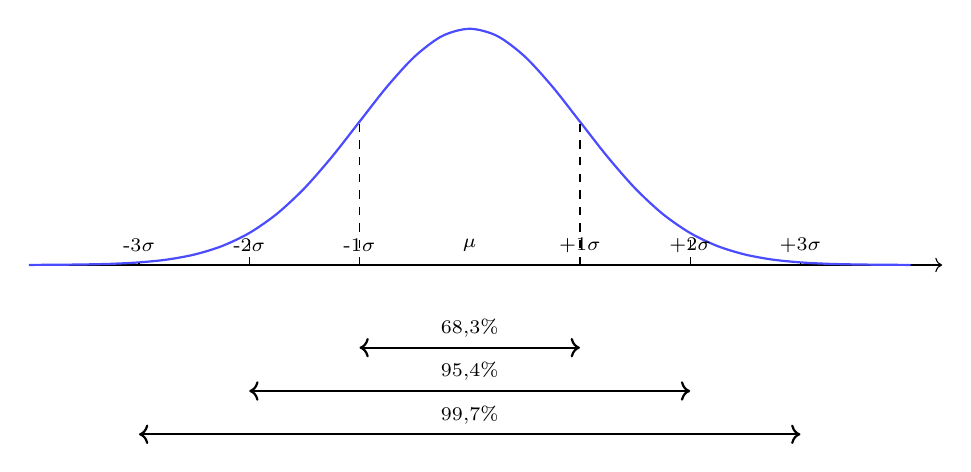
\begin{tikzpicture}
\draw[->] (0,0) -- (11.6,0); \draw[thick, blue!70] plot[smooth] coordinates {(0.00,0.001) (0.35,0.003) (0.70,0.007) (1.05,0.015) (1.40,0.033) (1.75,0.068) (2.10,0.132) (2.45,0.239) (2.80,0.406) (3.15,0.649) (3.50,0.974) (3.85,1.374) (4.20,1.820) (4.55,2.265) (4.90,2.647) (5.25,2.908) (5.60,3.000) (5.95,2.908) (6.30,2.647) (6.65,2.265) (7.00,1.820) (7.35,1.374) (7.70,0.974) (8.05,0.649) (8.40,0.406) (8.75,0.239) (9.10,0.132) (9.45,0.068) (9.80,0.033) (10.15,0.015) (10.50,0.007) (10.85,0.003) (11.20,0.001)};
\draw[dashed] (4.20,0) -- (4.20,1.82); \draw[dashed] (7.00,0) -- (7.00,1.82);
\draw[<->, thick] (4.20,-1.05) -- (7.00,-1.05) node[midway, above, font=\scriptsize] {68,3\%};
\draw[dashed] (2.80,0) -- (2.80,0.41); \draw[dashed] (8.40,0) -- (8.40,0.41);
\draw[<->, thick] (2.80,-1.60) -- (8.40,-1.60) node[midway, above, font=\scriptsize] {95,4\%};
\draw[dashed] (1.40,0) -- (1.40,0.03); \draw[dashed] (9.80,0) -- (9.80,0.03);
\draw[<->, thick] (1.40,-2.15) -- (9.80,-2.15) node[midway, above, font=\scriptsize] {99,7\%};
\node[font=\scriptsize] at (1.40,0.25) {-3$\sigma$};
\node[font=\scriptsize] at (2.80,0.25) {-2$\sigma$};
\node[font=\scriptsize] at (4.20,0.25) {-1$\sigma$};
\node[font=\scriptsize] at (5.60,0.25) {$\mu$};
\node[font=\scriptsize] at (7.00,0.25) {+1$\sigma$};
\node[font=\scriptsize] at (8.40,0.25) {+2$\sigma$};
\node[font=\scriptsize] at (9.80,0.25) {+3$\sigma$};

\end{tikzpicture}
\end{document}
